\ifdefined\XeTeXversion\else
  \pdfoutput=1
\fi
\documentclass[11pt]{article}

\usepackage[a4paper,margin=2.35cm]{geometry}
\usepackage[T1]{fontenc}
\ifdefined\XeTeXversion\else
  \usepackage[utf8]{inputenc}
\fi
\usepackage{lmodern}
\usepackage{microtype}
\usepackage{amsmath,amssymb,mathtools,bm}
\usepackage{booktabs,array,tabularx}
\usepackage{graphicx}
\usepackage{xcolor}
\usepackage{enumitem}
\usepackage{caption}
\usepackage{hyperref}
\usepackage{cleveref}

\hypersetup{
  colorlinks=true,
  linkcolor=blue!55!black,
  citecolor=teal!55!black,
  urlcolor=blue!65!black,
  pdftitle={Finite Predictivity Gates for Target-Free G2 Flavor Dynamics},
  pdfauthor={Matthew Connelly}
}

\newcommand{\Gr}{\operatorname{Gr}}
\newcommand{\Tr}{\operatorname{Tr}}
\newcommand{\rank}{\operatorname{rank}}
\newcommand{\diag}{\operatorname{diag}}
\newcommand{\SU}{\mathrm{SU}}
\newcommand{\SO}{\mathrm{SO}}
\newcommand{\OO}{\mathrm{O}}
\newcommand{\GeV}{\,\mathrm{GeV}}
\newcommand{\dd}{\mathrm{d}}
\newcommand{\status}[1]{\textsc{#1}}

\title{\textbf{Finite Predictivity Gates for Target-Free $G_2$ Flavor Dynamics}\\[0.35em]
\large Vacuum isolation, lepton mixing, and the boundary to an $E_6$ neutral sector}
\author{Matthew Connelly\\\small Independent Researcher}
\date{14 July 2026}

\begin{document}
\maketitle

\begin{abstract}
We test whether a finite class of target-free exceptional-geometric actions can select a physically meaningful three-family vacuum.  Four real three-planes in $\mathbb R^7$ define a configuration in $\Gr(3,7)^4$; a fixed unit vector reduces $G_2$ to a residual $\SU(3)$, and octonionic tensors generate the scalar action and signed-associator mass maps.  In a locked 74-action ensemble built from 21 normalized projector invariants, 68 branches pass a strict stationarity and stability cut and 29 are isolated modulo the known residual orbit.  Of the six isolated branches with full-rank mass maps in both sectors, none has two adjacent decade-scale singular-value gaps, while a CKM/PMNS-like matrix is not gauge defined under the independent left-frame basis freedoms.

We then test two remedies.  First, the unique primitive chiral loop and the unique lowest-degree exchange-even product within a three-channel complex-loop class are both locally stable, but retain seven and six physical zero modes, respectively.  Second, a shared auxiliary $U(3)$ link can be eliminated analytically to produce a nuclear-norm backreaction.  In a value-blind but structurally post-exposure extension of the 74 actions, 21 retained branches admit a lepton-angle diagnostic.  Sixteen have smooth classical quotient Hessians; all are stable and two are isolated, yet none lies inside all three NuFIT~6.0 three-sigma angle intervals.  The smallest best-fit $L^1$ angle residual is $22.62^\circ$ and occurs on a non-isolated branch.  Direct second-order automatic differentiation reproduces the smooth spectra to a maximum sorted discrepancy of $2.20\times10^{-6}$.  Five further branches are rank deficient, where the nuclear norm is nonsmooth and a classical Hessian is not defined.

These are negative finite gates, not a global no-go theorem.  They localize the missing structure: scalar closed-overlap invariants and a singular-value-only link do not provide a nondegenerate family-axis selector.  A separate appendix reanalyzes an external two-family supersymmetric $E_6$ benchmark, distinguishing the right-handed neutrino from the additional $E_6$ singlet; those fitted heavy scales are not derived from the $G_2$ construction.
\end{abstract}

\section{Introduction}

Exceptional groups provide rigid algebraic structures that can sharply constrain model building.  The octonions furnish the invariant three-form of $G_2$ and its dual four-form~\cite{Baez2002,Bryant1987}; fixing a unit imaginary direction leaves an $\SU(3)$ stabilizer and a natural complex structure on the orthogonal six-plane.  These ingredients make $G_2$ geometry a plausible laboratory for asking a precise question: can flavor structure be selected by geometry before observed masses and mixing data are supplied?

That question is stricter than obtaining a good numerical fit.  A predictive construction must specify its action without flavor targets, find stationary vacua, establish local stability, quotient all known continuous symmetries, and only then open mass or mixing observables.  Failure at any earlier stage prevents a later numerical matrix from being called a prediction.  The distinction is especially important for flavor, where unconstrained basis choices can generate apparently realistic mixing matrices without changing any invariant content.

This paper applies that gate discipline to a concrete four-plane $G_2$ model.  It consolidates three computational stages:
\begin{enumerate}[leftmargin=2.1em]
  \item a projector-invariant baseline and a signed-associator mass diagnostic;
  \item scalar complex-loop actions designed to correlate all four frames;
  \item an auxiliary unitary link whose exact elimination backreacts on the vacuum and permits a shared-space lepton-angle diagnostic.
\end{enumerate}
The central result is negative but specific.  Stable vacua are abundant, but predictivity fails in three distinguishable ways: the baseline lacks a gauge-defined relative left basis; scalar loops retain physical flat directions; and the integrated link stabilizes some branches without selecting observed lepton angles.

A short appendix addresses a separate neutral-fermion question raised by an $E_6$ benchmark.  It is deliberately not merged into the derivation chain: the $E_6$ masses are reproduced from published fitted parameters, whereas the $G_2$ gates are local computations in the four-plane model.

\subsection{Claim-status convention}

We use the evidence labels in \cref{tab:status}.  They are part of the scientific statement, not editorial decoration.

\begin{table}[t]
\centering
\caption{Evidence labels used throughout the paper.}
\label{tab:status}
\begin{tabularx}{\textwidth}{@{}>{\raggedright\arraybackslash}p{0.29\textwidth}X@{}}
\toprule
Label & Meaning \\
\midrule
\status{Analytic construction} & Follows from an explicit definition or finite algebraic argument. \\
\status{Verified computation} & Reproduced by retained code and machine-readable artifacts, with stated tolerances. \\
\status{Negative finite gate} & Rules out only the declared action class, starts, operators, and thresholds. \\
\status{Post-hoc diagnostic} & Evaluated after structural development; informative but not a held-out prediction. \\
\status{External benchmark} & Reanalysis of published fitted inputs, not a consequence of the local model. \\
\bottomrule
\end{tabularx}
\end{table}

No result below establishes a Standard Model derivation, a global classification of the invariant ring, or a proof that unobserved stationary branches do not exist.  In particular, a supplied two-page narrative invoking a ``Quaternionic Kernel Theorem'' contained neither a precise theorem nor a reproducible proof of its quoted CKM and PMNS numbers.  Those assertions are not used here.

\section{Exceptional-geometric setup}
\label{sec:setup}

\subsection{Octonionic tensors and four three-planes}

Let $\phi_{ijk}$ denote the standard octonionic $G_2$ three-form on $\mathbb R^7$, and let
\begin{equation}
  \Phi_{ijkl}=(*\phi)_{ijkl}
\end{equation}
be its Hodge dual.  We fix a unit vector $h=e_7$.  The stabilizer of $(\phi,h)$ is $\SU(3)$.  On $h^\perp$, define
\begin{equation}
  (J_h)_{ij}=\phi_{ijk}h_k,\qquad
  P_h=I-hh^{\mathsf T}.
  \label{eq:Jh}
\end{equation}
The identities
\begin{equation}
  J_h h=0,\qquad J_h^2=-P_h
  \label{eq:complex-identity}
\end{equation}
make $J_h$ a complex structure on the six-plane $h^\perp$.

The dynamical variables are four Stiefel frames
\begin{equation}
  X_a\in\mathbb R^{7\times 3},\qquad X_a^{\mathsf T}X_a=I_3,
  \qquad a=0,1,2,3,
\end{equation}
interpreted as
\begin{equation}
  (X_0,X_1,X_2,X_3)=(L_e,R_e,L_\nu,R_\nu).
\end{equation}
Their projectors $P_a=X_aX_a^{\mathsf T}$ are invariant under the frame gauges $X_a\mapsto X_aO_a$, $O_a\in\OO(3)$.  The physical configuration space of the baseline action is therefore $\Gr(3,7)^4$, with 48 local Grassmann coordinates before quotienting the residual $\SU(3)$ orbit.

For later mass diagnostics, the octonionic associator is represented by
\begin{equation}
  [e_a,e_b,e_c]=A_{abc}{}^d e_d,
  \qquad
  A_{abc}{}^d
  =\phi_{abm}\phi_{mc}{}^d-\phi_{bcm}\phi_{am}{}^d.
  \label{eq:associator}
\end{equation}
All tensor conventions were checked against direct octonion multiplication before optimization.

\subsection{Target-free scalar actions}

A finite scalar basis was assembled from contractions of $P_a$, $h$, $\phi$, and $\Phi$.  It contains single-frame, pair, triple, and four-frame structures, including traces such as $\Tr(P_aP_b)$ and $\Tr(P_aP_bP_aP_b)$ and tensor contractions of $\phi$ and $\Phi$ with projected indices.  Numerical rank-revealing decomposition on a locked Haar sample selected 21 independent feature directions.  Each feature was standardized by its sample mean and standard deviation.

The coefficient ensemble contained 74 actions: the positive and negative directions of each primitive feature and pair-sector combinations, together with 32 seeded Rademacher sign vectors normalized in coefficient space.  The coefficients and Haar normalization were frozen before any flavor diagnostic.  This is a finite computational design, not a basis theorem for all $G_2$ invariants.

For each action, four generic starts were optimized on the Stiefel product.  A branch was called stationary when the projected gradient norm was below $10^{-5}$.  The 48-dimensional local Hessian was classified using thresholds
\begin{equation}
  \lambda<-10^{-5}\quad\text{negative},\qquad
  |\lambda|\le 10^{-5}\quad\text{zero}.
  \label{eq:hessian-thresholds}
\end{equation}
The tangent orbit generated by the eight-dimensional residual $\SU(3)$ was constructed explicitly at every vacuum.  A stable branch is isolated only when its Hessian kernel contains no directions beyond that orbit.

\section{Baseline predictivity gate}
\label{sec:baseline}

\subsection{Vacuum stability and isolation}

At the strict reliability cut, 68 of the 74 action branches were stationary and stable, and 29 were isolated modulo the explicitly constructed residual orbit.  These counts differ slightly from a raw Hessian-only classification because the strict cut also excludes a numerically unreliable stationary representative.  The search used the best retained representative among four starts and therefore does not certify that every stationary branch has been found.

\begin{figure}[t]
  \centering
  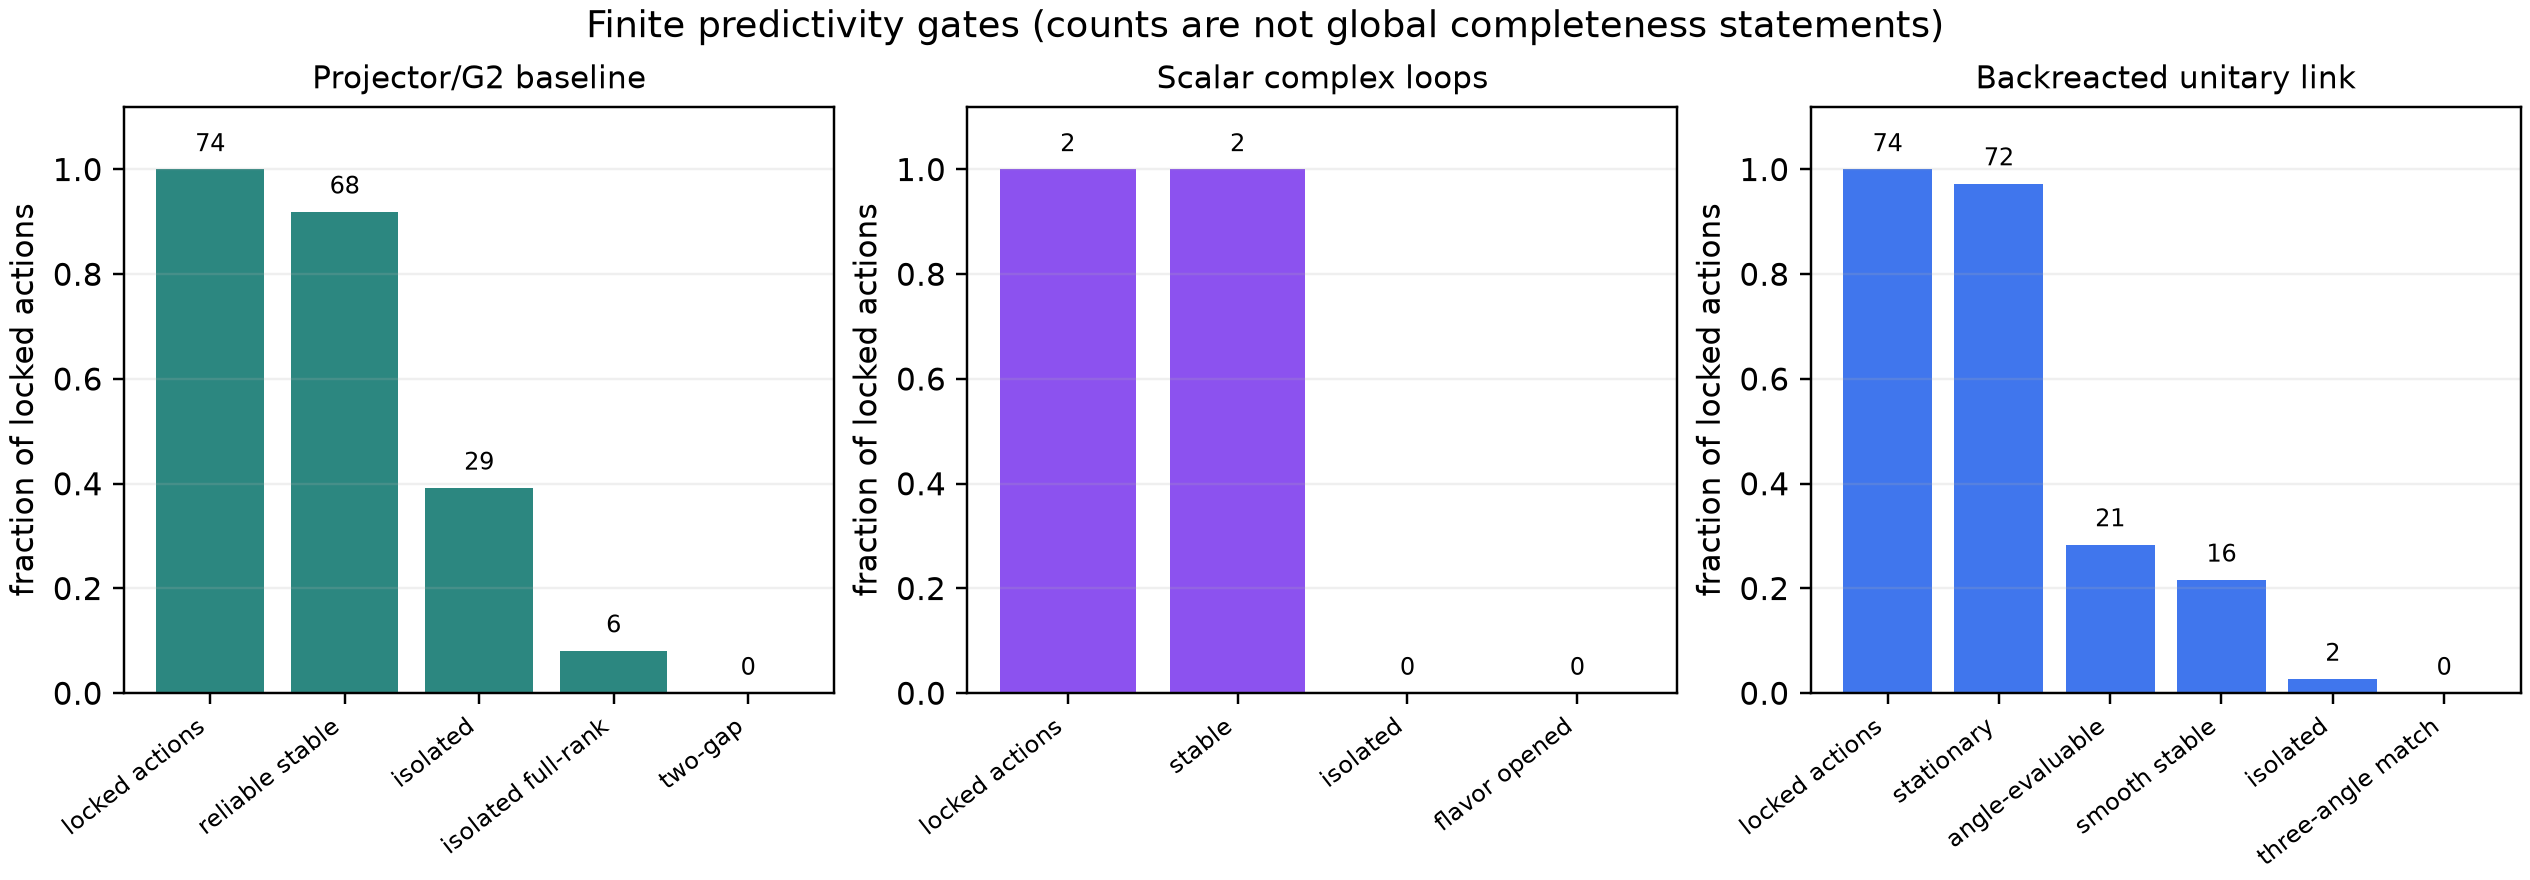
\includegraphics[width=0.95\textwidth]{predictivity_gate_summary_v1.png}
  \caption{Finite gate counts for the three action classes.  Bar heights are normalized by the number of locked actions in each panel, while integers give raw counts.  The stages are not global completeness statements and the two-loop panel contains only two symmetry-selected candidate actions.}
  \label{fig:gate-summary}
\end{figure}

\subsection{Signed-associator mass map}

Flavor was opened only after stationarity, stability, and degeneracy classification.  A composite direction was declared by
\begin{equation}
  V=\text{top eigenvector of}\quad
  P_h\left(\sum_{a=0}^{3}P_a\right)P_h,
  \label{eq:composite-v}
\end{equation}
provided that the top spectral gap exceeded $10^{-8}$.  For a left/right pair $(L,R)$, the signed-associator matrix was
\begin{equation}
  Y_{ij}=\left\langle [L_i,V,h],R_j\right\rangle.
  \label{eq:yukawa-map}
\end{equation}
Its singular values are invariant under the independent frame gauges.  Thirty-six reliable stable branches had a usable composite direction; 11 of those were isolated, and six were isolated with full-rank maps in both sectors.

An earlier endpoint-span count can mistake a single large gap for a three-rung hierarchy.  We therefore required both adjacent singular-value gaps to exceed one decade in each sector.  None of the six isolated, full-rank two-sector branches passed.  This is the first negative finite gate:
\begin{quote}
\status{Negative finite gate.} No isolated, full-rank, two-gap hierarchy occurs in the tested 74-action ensemble with the declared composite-$V$ signed-associator map.
\end{quote}
It is not a no-go theorem for another mass operator or for the full invariant ring.

\subsection{Why baseline mixing is undefined}

Let $Y_e$ and $Y_\nu$ be the two real $3\times3$ matrices obtained from \cref{eq:yukawa-map}.  A formal mixing proxy formed from their left singular vectors changes under the independent frame transformations
\begin{equation}
  L_e\mapsto L_e O_e,\qquad L_\nu\mapsto L_\nu O_\nu.
\end{equation}
The singular values are unchanged, but the relative left basis is arbitrary.  Consequently a CKM/PMNS-like matrix is not a physical observable of the baseline action.  This is a structural obstruction, not a failure to choose a preferred singular-value convention.

\section{Complex overlap and scalar loop actions}
\label{sec:loops}

The exceptional complex structure in \cref{eq:Jh} defines complex overlaps
\begin{equation}
  K_{ab}=X_a^{\mathsf T}(P_h+iJ_h)X_b.
  \label{eq:Kab}
\end{equation}
Up to a factor of two, $P_h+iJ_h$ is a rank-three complex projector on the complexified six-plane.  The frame transformations act as
\begin{equation}
  K_{ab}\mapsto O_a^{\mathsf T}K_{ab}O_b,
\end{equation}
so traces around closed frame cycles are gauge invariant.

\subsection{Three primitive oriented cycles}

There are three inequivalent oriented four-cycle pseudoscalars in the declared class:
\begin{align}
 I_1&=\Im\Tr(K_{01}K_{12}K_{23}K_{30}),\nonumber\\
 I_2&=\Im\Tr(K_{01}K_{13}K_{32}K_{20}),\nonumber\\
 I_3&=\Im\Tr(K_{02}K_{21}K_{13}K_{30}).
 \label{eq:loops}
\end{align}
Their characters are shown in \cref{tab:loop-characters}.  Complex conjugation reverses all three signs.

\begin{table}[t]
\centering
\caption{Discrete characters of the three primitive loop channels.}
\label{tab:loop-characters}
\begin{tabular}{@{}cccc@{}}
\toprule
Channel & sector exchange & left/right exchange & CP \\
\midrule
$I_1$ & $+1$ & $-1$ & $-1$ \\
$I_2$ & $-1$ & $-1$ & $-1$ \\
$I_3$ & $-1$ & $+1$ & $-1$ \\
\bottomrule
\end{tabular}
\end{table}

Requiring sector-even, left/right-odd, and CP-odd character selects the primitive action
\begin{equation}
  V_\chi=-\chi\,\frac{I_1}{\sigma_1},\qquad \chi=+1,
  \label{eq:vchi}
\end{equation}
within this finite class.  The opposite sign is the CP-conjugate convention.  After the primitive candidate failed isolation, the lowest-degree monomial containing all three characters and even under both exchanges was
\begin{equation}
  V_3=-\chi
  \left(\frac{I_1}{\sigma_1}\right)
  \left(\frac{I_2}{\sigma_2}\right)
  \left(\frac{I_3}{\sigma_3}\right),
  \label{eq:v3}
\end{equation}
where the locked Haar standard deviations are
\begin{equation}
  (\sigma_1,\sigma_2,\sigma_3)
  =(0.2786481,0.2812664,0.2736715).
\end{equation}
``Unique'' here means unique under the stated character and degree restrictions, not unique in the complete invariant ring.

\subsection{Quotient-Hessian result}

Each action was solved from 96 generic starts.  Every retained start approached the same numerical energy for its action, but this empirical convergence is not a proof of global minimality.  The local results are in \cref{tab:loop-gate}.

\begin{table}[t]
\centering
\caption{Quotient-isolation gates for the two scalar complex-loop actions.  Eigenvalue counts use the tolerances in \cref{eq:hessian-thresholds}.}
\label{tab:loop-gate}
\begin{tabular}{@{}lrrrrr@{}}
\toprule
Action & $\|\nabla V\|$ & negative & zero & positive & extra physical zero \\
\midrule
$V_\chi$ & $3.07\times10^{-14}$ & 0 & 15 & 33 & 7 \\
$V_3$    & $1.50\times10^{-11}$ & 0 & 14 & 34 & 6 \\
\bottomrule
\end{tabular}
\end{table}

Both stationary representatives are stable within tolerance.  Neither is isolated after subtracting the rank-eight residual $\SU(3)$ orbit.  The three-channel product reduces the number of extra physical zero modes from seven to six, but does not eliminate the continuous ambiguity.  Flavor was therefore not opened on either vacuum.

\section{Auxiliary unitary link and exact backreaction}
\label{sec:link}

\subsection{Shared left-generation space}

To compare the charged-lepton and neutrino left spaces, introduce a bifundamental link $\Sigma\in U(3)$ and define
\begin{equation}
  K\equiv K_{02}=L_e^{\mathsf T}(P_h+iJ_h)L_\nu.
  \label{eq:leftK}
\end{equation}
Under full-rank frame changes,
\begin{equation}
  K\mapsto O_e^{\mathsf T}KO_\nu,
  \qquad
  \Sigma\mapsto O_e^{\mathsf T}\Sigma O_\nu.
\end{equation}
The auxiliary interaction is
\begin{equation}
  V_{\mathrm{aux}}(\Sigma,K)=-\Re\Tr(\Sigma^\dagger K).
  \label{eq:vaux}
\end{equation}
If $K=U\,\diag(s_1,s_2,s_3)V^\dagger$ is a singular-value decomposition, the minimum is attained by the polar factor $\Sigma=UV^\dagger$ and
\begin{equation}
  \min_{\Sigma\in U(3)}V_{\mathrm{aux}}=-\sum_i s_i=-\|K\|_*.
  \label{eq:nuclear}
\end{equation}
Thus the link can be integrated out exactly.  The result is invariant under the independent frame gauges, but it depends only on the singular geometry of $K$.
For rank-deficient $K$, the minimum value remains well defined but the unitary polar completion is not unique; mixing angles obtained from a particular null-space completion are therefore not physical diagnostics.

For a locked standardized baseline action $V_c$, the tested backreacted action was
\begin{equation}
  V_{\mathrm{tot}}
  =V_c-\frac{\|K\|_*-\mu_K}{\sigma_K},
  \qquad
  \mu_K=0.3520919,\quad \sigma_K=0.3704670.
  \label{eq:vtotal}
\end{equation}
The coefficient $-1$ is a standardized modeling convention.  It is not derived from a coupling unification or a representation-theoretic normalization.  No PMNS angle or mass enters \cref{eq:vtotal}, but the link architecture was introduced after the baseline mixing obstruction was known.  We therefore call the extension \emph{value-blind but structurally post-exposure}, rather than a fully held-out prediction.

\subsection{Lepton-angle diagnostic}

For each sector, define the positive left operator
\begin{equation}
  J_f=Y_fY_f^\dagger.
\end{equation}
The neutrino operator is transported into the charged-lepton left space with $\Sigma$.  If $U_e$ and $U_\nu$ diagonalize the corresponding operators in their native spaces, the shared-space mixing matrix is
\begin{equation}
  U_{\ell}=U_e^\dagger\Sigma U_\nu.
  \label{eq:mixing}
\end{equation}
Its absolute values and rephasing invariants are physical under the frame gauges; raw matrix entries remain subject to conventional phases and permutations.  The three standard angles are extracted from $|U_{\ell,13}|$, $|U_{\ell,12}|$, and $|U_{\ell,23}|$ in a fixed mass ordering, while the Jarlskog invariant is
\begin{equation}
  J=\Im(U_{11}U_{22}U_{12}^*U_{21}^*)
  \label{eq:jarlskog}
\end{equation}
following the usual rephasing-invariant construction~\cite{KobayashiMaskawa1973,Jarlskog1985}.

The numerical comparison uses the normal-ordering NuFIT~6.0 analysis with atmospheric information~\cite{Esteban2024}.  The best-fit angles are
\begin{equation}
  (\theta_{12},\theta_{23},\theta_{13})=(33.68^\circ,43.3^\circ,8.56^\circ),
\end{equation}
with three-sigma intervals
\begin{equation}
  [31.63,35.95]^\circ,\quad [41.3,49.9]^\circ,\quad [8.19,8.89]^\circ.
  \label{eq:nufit-ranges}
\end{equation}
Although the benchmark also records $\delta_{\rm CP}$, the present gate scores only the three angles.  We therefore use ``three-angle compatible,'' not ``PMNS compatible,'' for a pass.

\section{Backreacted quotient-Hessian gate}
\label{sec:backreacted-results}

\subsection{Smooth, saturated, and nonsmooth branches}

The 74 backreacted actions were solved from four generic starts each; 72 had a retained stationary representative.  Requiring a usable composite direction and nondegenerate two-sector mass spectra left 21 angle-evaluable branches.  Their Hessian treatment splits into three cases:
\begin{enumerate}[leftmargin=2.1em]
  \item five unitary-saturated branches, evaluated with the exact second-order germ of the nuclear norm;
  \item eleven full-rank, nonunitary branches, evaluated by centered finite differences of the true-SVD gradient and independently by direct second-order automatic differentiation through the SVD;
  \item five rank-deficient branches, where the nuclear norm is nonsmooth and no classical Hessian is assigned.
\end{enumerate}
For the smooth branches, the residual $\SU(3)$ orbit was projected out before eigendecomposition.  The independent verifier reproduced all 16 smooth classifications and the five nonsmooth identifications.  The maximum discrepancy between sorted finite-difference and direct-autograd spectra was $2.20\times10^{-6}$, below the declared $2\times10^{-5}$ comparison tolerance.

\subsection{Angle and isolation results}

\begin{table}[t]
\centering
\caption{Backreacted lepton-angle and quotient-Hessian gate.  ``N/A'' marks rank-deficient branches at which the nuclear norm is nonsmooth.}
\label{tab:link-counts}
\begin{tabular}{@{}lr@{}}
\toprule
Gate quantity & Count \\
\midrule
locked actions & 74 \\
retained stationary actions & 72 \\
angle-evaluable branches & 21 \\
smooth classical Hessians & 16 \\
rank-deficient/nonsmooth & 5 \\
quotient-stable smooth branches & 16 \\
quotient-isolated smooth branches & 2 \\
three-angle-compatible and stable & 0 \\
\bottomrule
\end{tabular}
\end{table}

Every smooth branch is stable within tolerance, but only two are isolated.  Those two isolated solutions have angle triples
\begin{align}
 &(5.105^\circ,3.263^\circ,0.300^\circ),
 &&\Delta_1=76.87^\circ,\nonumber\\
 &(0.00058^\circ,1.774^\circ,0.00078^\circ),
 &&\Delta_1=83.77^\circ,
 \label{eq:isolated-angles}
\end{align}
where
\begin{equation}
  \Delta_1=\sum_{ij\in\{12,23,13\}}
  |\theta_{ij}-\theta_{ij}^{\mathrm{NuFIT\ best}}|.
\end{equation}
The closest retained branch has
\begin{equation}
  (\theta_{12},\theta_{23},\theta_{13})
  =(16.889^\circ,42.683^\circ,13.773^\circ),
  \qquad \Delta_1=22.622^\circ,
  \label{eq:best-angles}
\end{equation}
with $J=0.01065$.  It is stationary and quotient-stable, but has 22 quotient zero modes and is therefore not isolated.

\begin{figure}[t]
  \centering
  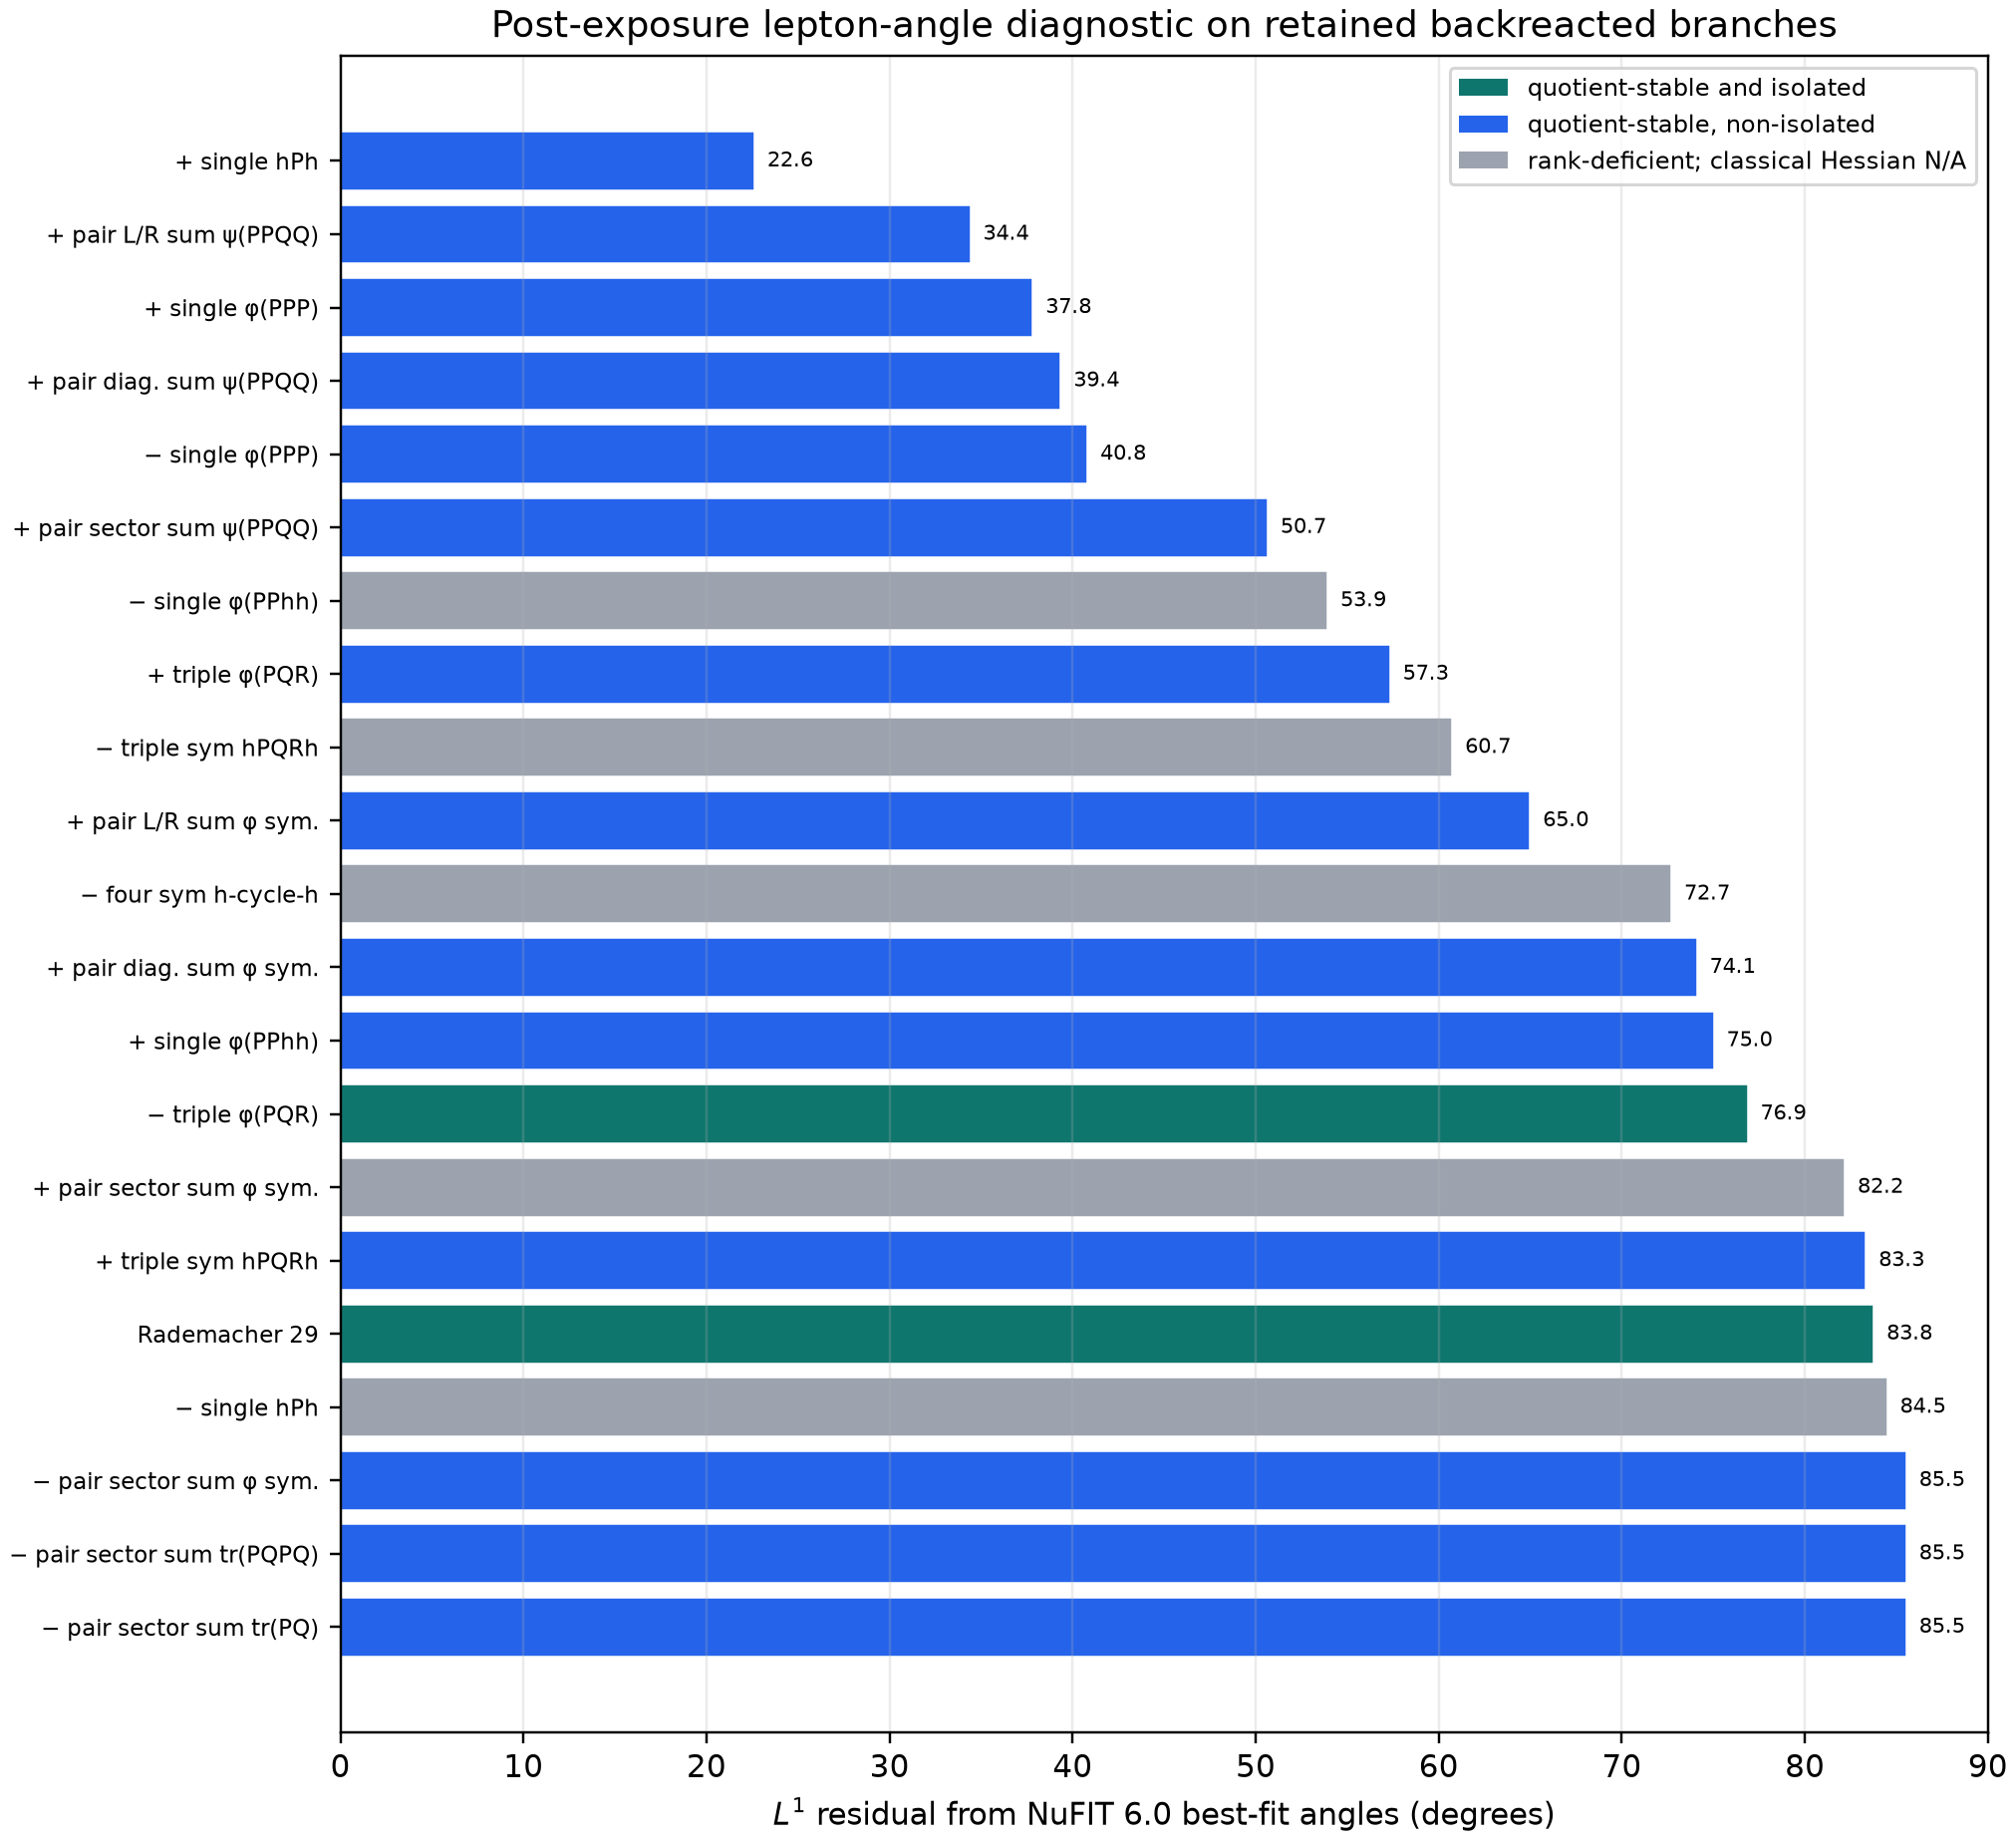
\includegraphics[width=0.98\textwidth]{pmns_angle_residuals_v2.png}
  \caption{Post-exposure three-angle diagnostics, sorted by $L^1$ residual from the NuFIT~6.0 best fit.  Blue bars are stable but non-isolated smooth branches and green bars are stable and isolated.  Gray bars are rank-deficient branches: the displayed values record the SVD convention used in the retained computation, but a classical Hessian is not defined and the unitary null-space completion is not unique.  The CP phase is not scored.}
  \label{fig:angle-residuals}
\end{figure}

The decisive result is therefore
\begin{quote}
\status{Independently verified negative finite gate.} Among the 16 smooth angle-evaluable branches found by the four-start 74-action solve, no quotient-stable branch lies inside all three NuFIT~6.0 three-sigma angle intervals.  Five additional rank-deficient branches are nonsmooth and are not assigned classical stability.
\end{quote}
The statement does not exclude an unobserved branch, another relative link coefficient, a different mass map, or an action outside the locked class.

\section{Structural interpretation}
\label{sec:interpretation}

The failures are informative because they occur at different gates.

First, projector-only scalar actions can isolate three-planes while leaving their internal left bases independent.  Mass singular values survive this gauge freedom; mixing does not.  Second, the complex loops in \cref{eq:loops} correlate all four frames, but scalar traces still leave continuous physical moduli.  Third, integrating out $\Sigma$ produces only $\|K\|_*$.  At unitary saturation, all three singular values of $K$ are fixed and the nuclear-norm term is constant over the reachable orientation family.  It can stabilize singular geometry without selecting the observed unitary orientation.

These observations point to a more specific missing object than simply ``more terms.''  A viable extension requires a matrix-valued family selector, say $T_L$, with a nondegenerate spectrum in the shared left-handed generation space.  Schematically one may consider
\begin{equation}
  V_{\mathrm{family}}
  =\sum_{f=e,\nu}
   \|T_LK_{L_fR_f}-K_{L_fR_f}T_{R_f}\|_F^2
  -\chi\,\Im\Tr\!\left(T_LK_{01}K_{12}K_{23}K_{30}\right).
  \label{eq:schematic-family}
\end{equation}
Equation~\eqref{eq:schematic-family} is a search direction, not a locked model.  To become predictive, the representation of $T_L$, its self-potential, the right-handed tensors, and every relative coefficient must be derived without flavor targets.  Its quotient Hessian must then leave only gauge or explicitly classified discrete degeneracies.

A concrete physical interpretation would be a dynamical family-order parameter shared by the charged-lepton and neutrino Yukawa sectors.  In a four-dimensional effective theory this could arise from an adjoint or higher-rank condensate; in a condensed-matter analogue it resembles a nondegenerate mode-splitting tensor that selects axes inside a degenerate multiplet.  The present scalar actions lack precisely that axis-resolving information.

\section{Limits of the calculation}
\label{sec:limits}

The following boundaries are essential.
\begin{enumerate}[leftmargin=2.1em]
  \item \textbf{Finite action class.}  The 21 features are numerically independent on a locked sample, but they do not constitute a theorem about the full invariant ring.
  \item \textbf{Finite starts.}  Four generic starts were used per baseline and backreacted action.  The loop candidates used 96 starts.  Neither protocol proves global completeness.
  \item \textbf{Local Hessians.}  Stability is local and tolerance dependent.  Rank-deficient nuclear-norm branches are nonsmooth and are not silently classified as stable or unstable.
  \item \textbf{Model-dependent mass map.}  The signed-associator map and composite direction in \cref{eq:composite-v,eq:yukawa-map} are declared diagnostics, not derived Standard Model Yukawa operators.
  \item \textbf{Post-exposure lepton test.}  No observed angle enters the backreacted objective, but the shared-link architecture was introduced to repair a known mixing obstruction.  The angle comparison is exploratory rather than a pristine blind prediction.
  \item \textbf{Angle-only score.}  The CP phase and oscillation mass splittings are not included in the compatibility gate.
  \item \textbf{No zero-parameter claim.}  Haar standardization fixes numerical scales for comparison, not physical coupling constants.  In particular, the relative coefficient of the nuclear term is assumed.
\end{enumerate}

\section{Conclusion}

The four-plane $G_2$ model passes several nontrivial mathematical and numerical checks: its tensor kernel is self-consistent, many locked scalar actions possess stable stationary vacua, some are isolated modulo the residual $\SU(3)$, closed complex overlaps have the required gauge and discrete characters, and the integrated unitary link admits independent second-order verification.  Those successes do not produce a flavor prediction.

The baseline action class fails to give both a three-rung hierarchy and a gauge-defined mixing matrix.  The two symmetry-selected scalar loop actions are stable but non-isolated.  The nuclear-norm backreaction produces 16 smooth stable lepton-angle branches, including two isolated branches, but none satisfies all three NuFIT~6.0 three-sigma angle intervals.  The closest branch is non-isolated and remains $22.62^\circ$ away in the angle-only $L^1$ diagnostic.

The appropriate conclusion is not that exceptional flavor geometry is impossible.  It is that this minimal scalar architecture lacks a nondegenerate family-axis selector.  A next model should derive such a matrix-valued order parameter first, pass stationarity and quotient-isolation gates without flavor data, and only then evaluate masses and mixing.

\appendix
\section{External \texorpdfstring{$E_6$}{E6} neutral-fermion benchmark}
\label{app:e6}

This appendix is a provenance-controlled reanalysis of the two-family fit in Ref.~\cite{BabuBajcSusic2015}.  It is not derived from the $G_2$ vacuum action.

Under
\begin{equation}
 E_6\supset \SO(10)\times U(1),\qquad
 \mathbf{27}=\mathbf{16}_{+1}\oplus\mathbf{10}_{-2}\oplus\mathbf{1}_{+4},
 \label{eq:e6-branching}
\end{equation}
the right-handed neutrino $\nu^c$ belongs to $\mathbf{16}_{+1}$, whereas the extra sterile fermion $s$ is the distinct $\SO(10)$ singlet in $\mathbf{1}_{+4}$.  The extra $U(1)$ charge in \cref{eq:e6-branching} is not $B-L$.

In the published neutral-fermion matrix, the corresponding Majorana subblocks are
\begin{equation}
  M_{\nu^c}=f_1Y_{351'},\qquad M_s=f_3Y_{351'}.
  \label{eq:e6-masses}
\end{equation}
The benchmark sets $f_2=0$, so these two singlet blocks do not mix at the quoted GUT-scale level.  Independent decimal and NumPy diagonalizations reproduce the positive masses in \cref{tab:e6-masses}.

\begin{table}[h]
\centering
\caption{Reproduced two-family fitted masses from Ref.~\cite{BabuBajcSusic2015}.  They are external benchmark values, not parameter-free predictions.}
\label{tab:e6-masses}
\begin{tabular}{@{}lcc@{}}
\toprule
Benchmark & $M_{\nu^c}$ physical masses $[\GeV]$ & $M_s$ physical masses $[\GeV]$ \\
\midrule
Point 1 & $1.49556\times10^{11},\ 1.52852\times10^{11}$
        & $6.6792\times10^{15},\ 6.8264\times10^{15}$ \\
Point 2 & $1.58424\times10^{12},\ 4.04616\times10^{12}$
        & $3.9606\times10^{15},\ 1.01154\times10^{16}$ \\
\bottomrule
\end{tabular}
\end{table}

The intermediate-scale $\nu^c$ states are the type-I seesaw candidates in this fit; the $s$ states lie near the unification scale.  Exact active--sterile admixtures cannot be reconstructed because the benchmark table omits the electroweak-doublet vacuum composition needed for the full neutral matrix.  A third-family spectrum is also absent.

Finally, the decomposition $\mathbf{16}+\mathbf{10}+\mathbf{1}$ has dimension 27.  It is the $E_6$ branching in \cref{eq:e6-branching}, not a branching of the $F_4$ fundamental $\mathbf{26}$.  Any local claim $\mathbf{26}\to\mathbf{16}+\mathbf{10}+\mathbf{1}$ therefore fails a dimensional gate.

\section{Numerical verification and artifact ledger}
\label{app:repro}

All optimization and Hessian calculations used double precision.  The retained workflow separates action locking, vacuum solving, quotient-Hessian classification, and flavor scoring.  The backreacted nonunitary Hessians were recomputed by direct second-order automatic differentiation through the true singular-value decomposition; the saturated unitary germ was verified separately; and rank-deficient points were recorded as nonsmooth rather than regularized into a classical Hessian.

The source distribution contains a machine-readable claim ledger with SHA-256 hashes for the authoritative JSON artifacts.  The principal artifact families are:
\begin{itemize}[leftmargin=2.1em]
  \item target-free action basis, vacuum, stability, post-stability flavor, and shape-verifier results;
  \item primitive and three-channel loop action locks, vacuum solves, and quotient-Hessian gates;
  \item backreacted link action lock, vacuum solve, angle-evaluable quotient-Hessian gate, and independent autograd verification;
  \item external $E_6$ benchmark inputs, spectra, and independent arithmetic verification.
\end{itemize}
The claim ledger also records excluded claims and the exact boundary of each finite gate.

\bibliographystyle{unsrt}
\bibliography{references_v2}

\end{document}
